\documentclass{amsart}

\usepackage{graphicx}
\usepackage{hyperref}

\title{CSCI 6907 Project Status Report\\
Lights Out Management}
\author{James Lee\\
\texttt{jameslee@gwu.edu}}
\date{\today}

\begin{document}
\maketitle

My original implementation plan called for the completion of the project by Mar 25, so when I say what I say next, I don't want it to seem as if my project was too easy or unchallenging.  I worked on it every weekend for almost two months.  The implementation phase of my project is complete.

\section{Changes}
My proposal called for using Telnet as the network protocol for my LOM.  After a lot of frustration trying to convert the VT100 escape commands to NVT escape commands, I discovered \href{http://www.ietf.org/rfc/rfc1282.txt}{Rlogin}, which is a lightweight remote terminal similar to Telnet, but it assumes like-to-like terminals, so escape commands can be passed-through unprocessed.  I modified my project to use the Rlogin protocol.

I also changed my project to use a third-party \href{http://www.freetronics.com/products/ethernet-shield-with-poe}{Ethernet Shield} which includes the \href{http://www.wiznet.co.kr/UpLoad\_Files/ReferenceFiles/W5100\_AN\_SPI.pdf}{SPI fixes} that would have made it impossible to use the official Arduino Ethernet Shield without hardware modification.

I was also able to implement the interface to be able to dynamically change the LOM's network settings, saving the settings persistently in EEPROM.

\section{Issues}
A remaining issue is that I cannot reliably operate my UART above 9600 baud while using the network interface.  I hope to be able to prove it in the final report, but the 16 MHz AVR on the Arduino seems to be too slow to move that much data very fast.  That said, 9600 baud is a perfectly workable speed for a failsafe console.  In fact, that's how high-end Sun servers' LOMs come configured out-of-the-box.

I'd also like to look into being able to disconnect clients after a certain timeout.

\section{Construction}
All of the components have been constructed on a bread-board and the code is complete (though it could use some clean-up and commenting).  You can view the code as of this writing at \url{https://github.com/MrStaticVoid/school/tree/e50721f4588ad0f41179d0e705f4caa33ed4ae4e/CSCI6907/project/sketch}.  Here is a photo of the current build:

\begin{center}
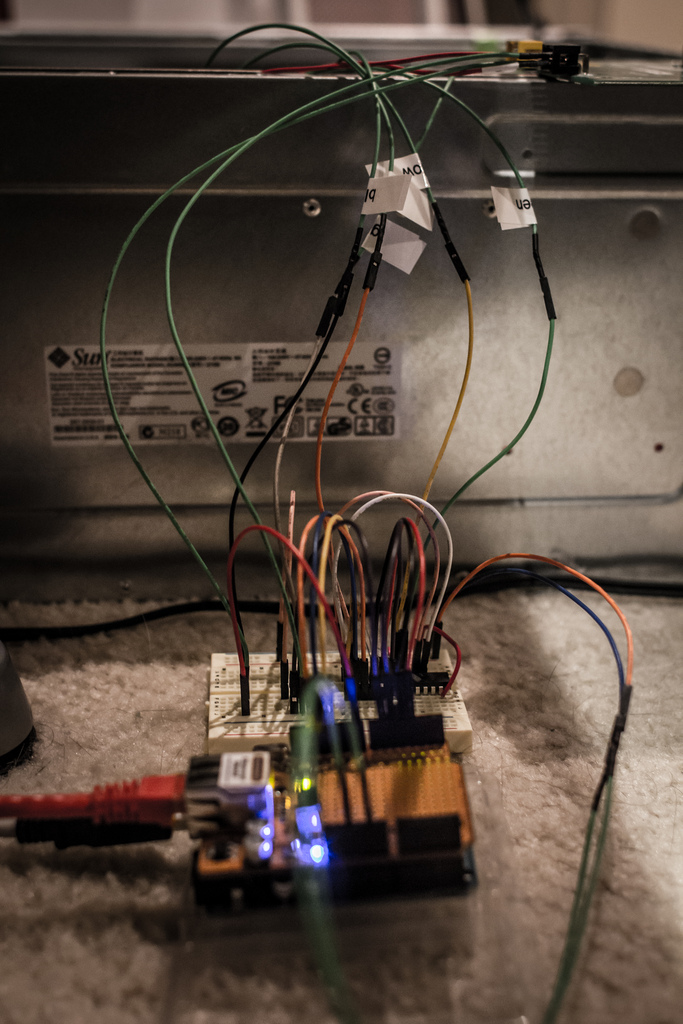
\includegraphics[width=.8\textwidth]{build.jpg}
\end{center}

The schematic remains largely unchanged from my proposal.  I did learn that the LED pins on the motherboard are reverse-biased (such that one pin always supplies current and the other goes high and low to turn the LED off and on).  That necessitated a change in my power-detection circuit from using two NPN transistors to one PNP transistor, and finally just a direct connection from the Arduino to the LED switching pin.  This is working well.

Time permitting, I hope to solder everything onto the prototyping area of the Ethernet Shield.  This is a rough drawing, just to show that everything should fit.  I need to rework it to reflect the simplified power-detection circuit:

\begin{center}
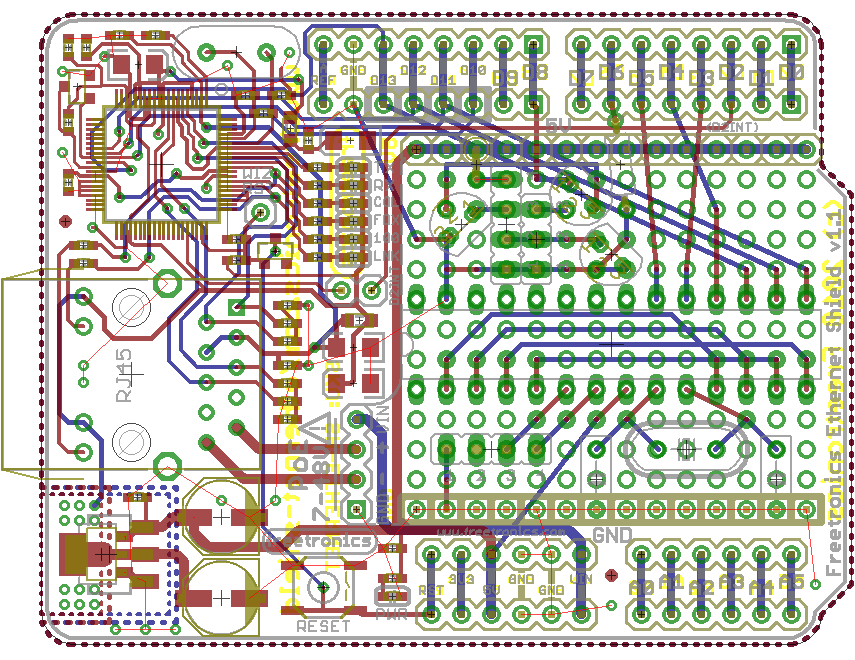
\includegraphics[width=.9\textwidth]{pcb.png}
\end{center}

\end{document}
